% !TeX encoding = utf8
% !TeX spellcheck = pl_PL

\documentclass[11pt, a4paper, twoside]{article}
\usepackage{graphicx, color, rotating} 
\usepackage[MeX, plmath]{polski} %MeX - tryb pełnej polonizacji
\usepackage[OT4]{fontenc} % T1 - skład fontami EC; OT4 - układ fontów PL
\usepackage{ae,aecompl}
\usepackage[utf8]{inputenc}
\usepackage{lmodern} %czcionka latin modern; jednolita dla tekstu i wzorów;
\usepackage{a4wide}
\usepackage{amsmath}
\usepackage{amssymb, latexsym}
\usepackage{array}
\usepackage{bm}
\usepackage[shortlabels]{enumitem}
\usepackage[font=footnotesize]{caption} %rozmiar czcionki podpisów pod rysunkami
\usepackage{float}
\usepackage{subfig} %obrazki obok siebie
\usepackage[hidelinks]{hyperref}
\usepackage{indentfirst}
\usepackage{geometry}
\geometry{left=25mm, right=25mm, top=25mm, bottom=25mm}

\usepackage[final]{pdfpages}
\usepackage{pdflscape}
\prefixing %notacja prefiksowa w pakiecie 'polski'
\frenchspacing
\linespread{1.1}
\renewcommand{\figurename}{Rys.}
%\renewcommand*\thesubsection{\arabic{subsection}} % zmiana numeracji podsekcji 0.X -> X

\begin{document}
	
	\begin{center} 
		{\Large Wydział Elektroniki i Technik Informacyjnych}
		\vskip0.2cm
		{\LARGE \textbf{Modelowanie i Symulacja Komputerowa (MISK): Smart City --~raport z etapu I projektu  } } 
		\vskip0.3cm
		{\Large Szymon Jarocki, Daniel Giełdowski, Maciej Kłos, Michał Okoński}
		\vskip0.8cm
	\end{center} 
	
	Celem etapu pierwszego projektu była analiza zagadnienia i przygotowanie środowiska roboczego. Kwestie te przedstawiono pokrótce w sekcjach nr \ref{sec:analiza} i~\ref{sec:przygotowanie}.	
	
	\section{Analiza zagadnienia}
	\label{sec:analiza}
	Zadanie polega na~zaprojektowaniu oraz zaimplementowaniu symulatora grupy autonomicznych samochodów (bez kierowcy), które mają poruszać się po ulicach pewnego miasta i~docierać pod zadane adresy. Wybrany został wariant sterowania autonomicznego, w~którym pojazdy same decydują o~swojej trasie, mając do~dyspozycji odpowiednie czujniki umożliwiające unikanie kolizji. Przyjmujemy, że po~drogach poruszają się jedynie rozważane pojazdy. Głównym celem sterowania --- oprócz jazdy bezkolizyjnej --- jest to, aby samochody osiągały swoje punkty docelowe jak najszybciej.
	
	Przy realizacji projektu wykorzystane zostaną środowiska V-REP i~MATLAB. Pierwsze z~nich posłuży do~symulacji poruszania się samochodów, natomiast drugie z~wymienionych będzie wykorzystane do~implementacji algorytmów wyznaczania tras dla pojazdów. Prace, które są do~wykonania można określić w~następującym porządku:
	\begin{enumerate}[1)]
		\item implementacja w symulatorze planu dzielnicy miasta przy zapewnieniu wystarczającego stopnia złożoności symulowanego ,,świata'',
		\item dobór algorytmów wyznaczania tras dla poruszających się pojazdów w~kontekście posiadanych przez nie czujników i~w~związku z~minimalizacją czasu osiągania punktów docelowych,
		\item implementacja wybranych algorytmów i~konsolidacja oprogramowania,
		\item testowanie poprawności działania symulatora i ocena optymalności rozwiązania.
	\end{enumerate}
	Co ważne, powyższa kolejność nie jest sekwencją, w~której kolejne etapy realizowane są dokładnie raz w~przedstawionej kolejności. Należy raczej zakładać postępowanie iteracyjne, wiążące się z~powrotem do~wcześniej wykonywanych zadań w~celu dokonania potrzebnych poprawek, które mogą przyczynić się do~uzyskania lepszego rozwiązania.
	
	\section{Przygotowanie środowiska roboczego}
	\label{sec:przygotowanie}
	Przygotowanie środowiska roboczego polegało przede wszystkim na~instalacji i~zapoznaniu się z~programem V-REP. Z~kolei pakiet MATLAB był już do~naszej dyspozycji z~racji wykonywania z~jego użyciem innych projektów. W~dalszej perspektywie konieczne będzie utrzymanie tych środowisk,  polegające m.in. na~dokonywaniu ewentualnych aktualizacji czy też konfiguracji przydatnych funkcjonalności.
	
	Prace przygotowawcze polegały także na~sprawdzeniu możliwości wspólnego zastosowania obu programów oraz na~przygotowaniu wstępnego planu dzielnicy miasta. Okazało się, że należy utworzyć własny plan z~racji trudności w~odnalezieniu istniejących już rozwiązań (o~ile takowe są), które można by odpowiednio zaadaptować na~potrzeby niniejszego projektu.
	
	\subsection{Instalacja}
	\label{subsec:instalacja}
	Uruchomienie pracy nad projektem wymagało instalacji dwóch programów: MATLAB oraz \mbox{V-REP}. Ze względu na aktualnie zainstalowane systemy operacyjne instalacja została wykonana na systemie Windows. Licencja programu MATLAB jest dla nas dostępna jako studentów Politechniki Warszawskiej. Przy instalacji tego oprogramowania nie zostały podjęte żadne niestandardowe kroki. Jeżeli chodzi o program V-REP, to z racji braku wykupionej licencji zdecydowaliśmy się na wersję V-REP PRO EDU udostępnioną przez producenta, która pozwala na~wykorzystywanie pełnych możliwości oprogramowania do~celów akademickich. Także w wypadku tej instalacji nie zostały podjęte żadne niestandardowe kroki.
	
	\subsection{Zapoznanie się ze środowiskiem i tworzenie świata}
	\label{subsec:scena}
	Jak już wcześniej stwierdziliśmy, środowisko MATLAB jest nam dobrze znane ze względu na~fakt wykonywania w nim innych projektów naukowych. Skupiliśmy się zatem na poznaniu oprogramowania V-REP. W tym celu utworzyliśmy w nim własny świat (zwany w środowisku \mbox{V-REP} sceną), na którym rozpoczęliśmy budowanie mapy. Jak wspomnieliśmy, mimo poszukiwań, nie udało nam się dotychczas znaleźć sposobu na udostępnienie programowi planów realnych miast (na przykład poprzez konwersję map dostępnych w internecie), co skłoniło nas do~podjęcia próby zbudowania swojego. Dotychczas udało nam się przetestować następujące funkcjonalności programu:
	\begin{itemize}
		\item dodawanie przeszkód statycznych (budynków oraz drzew),
		\item wstawianie dróg i dostosowanie ich koloru (w formie płaszczyzn),
		\item dodawanie pojazdów (dostępny w programie V-REP model pojazdu o napędzie Ackermanna),
		\item uruchamianie symulacji,
		\item sterowanie pojazdami (na razie egzekwowane za pomocą klawiatury),
		\item obecność kolizji pojazdów z otoczeniem i ze sobą nawzajem.
	\end{itemize}
	
	\subsection{Integracja oprogramowania}
	\label{subsec:integracja}
	Ważnym aspektem projektu jest połączenie symulacji działającej w programie V-REP ze~sterowaniem egzekwowanym za pomocą algorytmów zaimplementowanych w MATLAB-ie. Jak okazało się, po krótkich poszukiwaniach, twórcy programu V-REP załączyli do swojego kilka przykładów takiego połączenia wraz z plikami umożliwiającymi pisanie własnych skryptów. W~celu ustanowienia połączenia należy wykonać następujące kroki:
	\begin{enumerate}[1)]
		\item Otworzyć odpowiednią scenę w programie V-REP (można skorzystać z istniejącego świata $remoteApiCommandServerExample.ttt$).
		\item Otworzyć odpowiedni port w programie V-REP poprzez dodanie odpowiedniego skryptu do sceny. W skrypcie należy także zawrzeć inne funkcje, które miałyby być wywoływane przez MATLAB-a.
		\item Utworzyć w programie MATLAB odpowiedni skrypt umożliwiający komunikację oraz zlecający wykonanie pożądanych działań, lub skorzystać z jednego z już istniejących.
		\item Skopiować następujące pliki z lokalizacji instalacji programu V-REP do folderu zawierającego wykonywany w~MATLAB-ie skrypt (lub dodać ich lokalizację do źródeł MATLAB-a):
		\begin{itemize}
			\item $..\backslash V-REP\_PRO\_EDU\backslash programming\backslash remoteApiBindings\backslash \\matlab\backslash matlab\backslash remApi.m$
			\item $..\backslash V-REP\_PRO\_EDU\backslash programming\backslash remoteApiBindings\backslash \\matlab\backslash matlab\backslash remoteApiProto.m$
			\item $..\backslash V-REP\_PRO\_EDU\backslash programming\backslash remoteApiBindings\backslash \\lib\backslash lib\backslash Windows\backslash 64Bit\backslash remoteApi.dll$
		\end{itemize}
		\item Uruchomić symulację w programie V-REP.
		\item Uruchomić skrypt sterujący MATLAB-a.
	\end{enumerate}
	Wykonując wspomniane akcje i używając dostępnych skryptów, udało nam się z powodzeniem przetestować działanie komunikacji pomiędzy obydwoma programami --- zarówno w scenie testowej udostępnionej przez deweloperów programu V-REP, jak i w utworzonej przez nas scenie z mapą. Skrypty testowe umożliwiły sprawdzenie następujących działań:
	\begin{itemize}
		\item wysyłanie danych z MATLAB-a do V-REP-a i z powrotem,
		\item wywoływanie przez program MATLAB funkcji udostępnionych przez V-REP,
		\item zdalne tworzenie i edycja obiektów na scenie,
		\item wysyłanie kodu wykonywalnego do V-REP-a i jego egzekucja,
		\item sterowanie wykonywaniem kroków symulacji oraz jej wyłączanie.
	\end{itemize}
	
	%\newpage
\section{Model pojazdu}
Na potrzeby symulacji utworzony został odpowiedni model samochodu. W tym celu wykorzystane zostały możliwości edycji obiektów dostępne w programie V-REP. Jako baza posłużył jeden z modeli, obecny w oprogramowaniu po jego instalacji, o nazwie 'simple Ackermann steering.ttm'. Model ten wyposażony był w funkcjonalne koła przymocowane do podstawy oraz podstawowe oprogramowanie umożliwiające sterowanie pojazdem z wykorzystaniem klawiatury.

W celu przystosowania modelu do naszych potrzeb wykonany został szereg akcji. Model upodobniono wyglądem do realnego pojazdu poprzez dodanie dodatkowych kształtów, co z pewnością pozytywnie wpłynie na wizualny odbiór symulacji. Dodane zostały między innymi atrapy takich elementów jak szyby, opony oraz reflektory. Z modelu zostały także usunięte zbędne elementy, takie jak linie pokazujące skręcenie osi poszczególnych kół podczas symulacji.

\begin{figure}[!h]
	\centering
	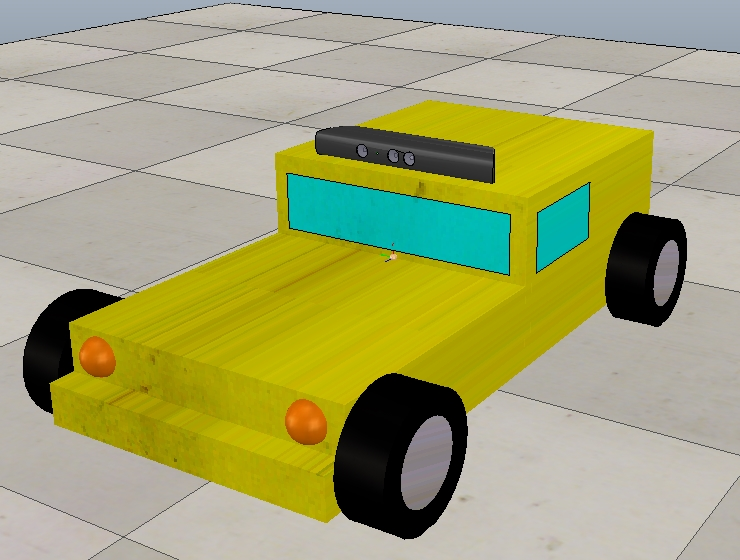
\includegraphics[width=.8\linewidth]{car.jpg}
	\caption{Model samochodu}
	\label{fig:model}
\end{figure}

Samochód biorący udział w symulacji jest z założenia pojazdem autonomicznym, o wysokim stopniu sztucznej inteligencji. Postrzega on swoje środowisko przez posiadane sensory i~na~podstawie danych identyfikuje wszystkie elementy otoczenia. Stworzenie takiego samochodu wymagałoby jednak ogromnych nakładów czasu i pracy, które są dla nas niedostępne z oczywistych względów. Z tego powodu zdecydowaliśmy się zastosować kilka uproszczeń. Obecny w symulacji model faktycznie posiada jedynie dwa rodzaje czujników: 14 czujników odległości oraz kamerę o niskiej rozdzielczości. Czujniki mają formę wskaźników laserowych, widocznych podczas symulacji, co umożliwia weryfikację poprawności ich działania. Są one rozmieszczone naokoło samochodu w rozkładzie: 2 z przodu, 2 z tyłu, po 3 na każdym boku i jeden na każdym rogu pojazdu. Czujniki zwracają odległość samochodu od innych nieprzenikalnych elementów symulacji, co umożliwia określenie czy przed lub za modelem znajduje się inny pojazd. Kamera zamieszczona na dachu pojazdu zwraca obraz RGB o niskiej rozdzielczości. Jeżeli pozwoli na~to~czas realizacji projektu, obraz ten wykorzystany zostanie do wykrywania aktualnego koloru sygnalizacji świetlnej. W przeciwnym wypadku stan świateł przekazywany będzie bezpośrednio do~wiadomości pojazdu. Inne czujniki, umożliwiające takie rzeczy, jak wykrywanie nawierzchni, identyfikację znaków drogowych oraz obserwację ruchu innych modeli znajdujących się w pobliżu, nie zostały fizycznie umieszczone ani zaimplementowane w modelu. Dane te przesyłane będą bezpośrednio z symulacji do poszczególnych pojazdów.

\begin{figure}[!h]
	\centering
	\subfloat[] {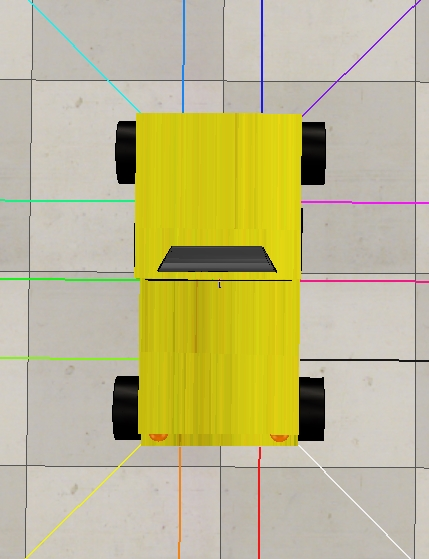
\includegraphics[width=.33\linewidth]{car_sensors.jpg}} \hspace{0.2cm}
	\subfloat[] {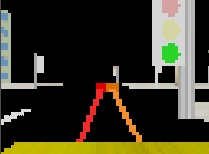
\includegraphics[width=.58\linewidth]{car_kinect.jpg}}
	\caption{Funkcjonalności pojazdu: (a) działanie czujników odległości, (b) obraz widziany z kamery.}
	\label{fig:model_fun}
\end{figure}

\end{document}

